\section{Analysis}


\subsection{Correctness}

In order to ensure the functional correctness of Online-FAST, we claim two important properties, and relevant proofs can refer to Appendix A.

\begin{theorem}[Fairness Degree Converges to Zero] Given the arriving probability $A$ for the user set, the sum of Top-N Fairness Degree of all the users in each round will approach to zero (i.e.  $\lim_{T \rightarrow \infty}\sum_{u_{i} \in U} F_{i}^{T}=0$) if and only if the users share a same arriving probability.
\label{thm1}
\end{theorem}

Theorem \ref{thm1} indicates that when considering arriving probability, the fairness degree should be calculated and maintained globally, no matter whether the user actually comes in the current round, and that the arriving probabilities for the users should be the same, otherwise our proposed fairness degree will lose the converge-to-zero property, thus failing to accurately describe the fairness of the recommendation system.

This property can be further illustrated by the two figures in \ref{fig:thm1}. We compare experiments on different strategies on users with the same arriving probability against users with diverse arriving probability. If the users have a different arriving probability, the preempt algorithm will not keep the average of fairness degree to zero.

\begin{figure}[htbp]
  \centering
  \subfigure{
    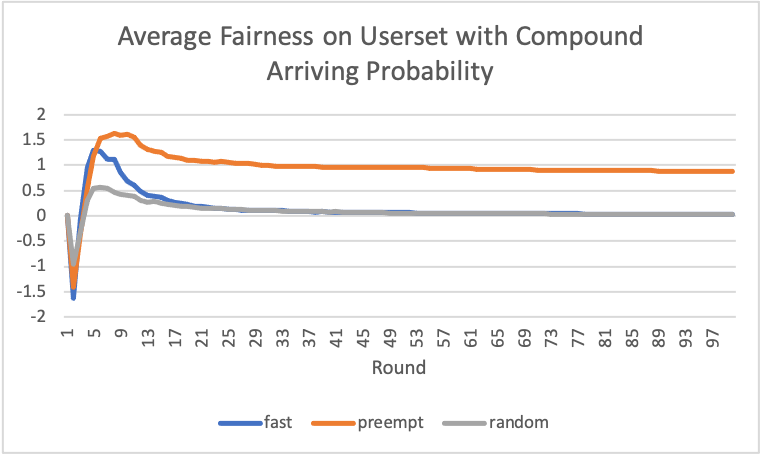
\includegraphics[scale=0.21]{img/thr1.png}}
  \hspace{0.1in} % 两图片之间的距离
  \subfigure{
    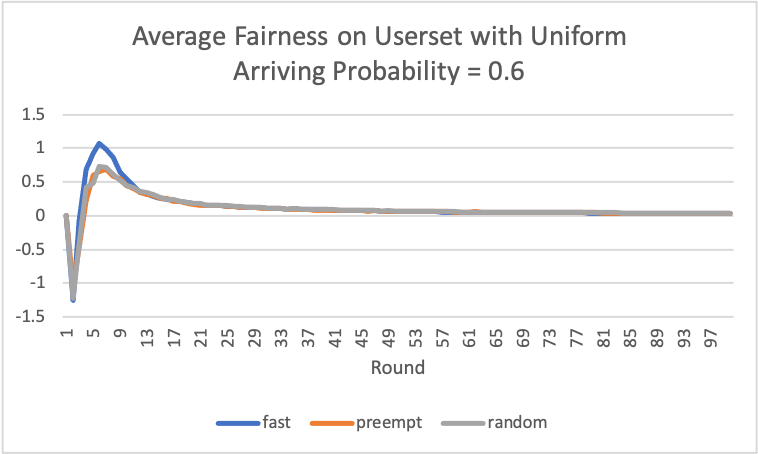
\includegraphics[scale=0.21]{img/thr2.png}}
  \caption{An intuitive interpretation of Theorem \ref{thm1}
  \label{fig:thm1}}
\end{figure}


Based on Theorem \ref{thm1}, we can argue the functional correctness of our online-FAST algorithm. Claim \ref{thm2} indicates F-FAST can assure long-term fairness for multi-round recommendations in an online scenario where users' arriving probabilities are given.


\begin{claim}[Variance Convergence] For a group of users with the same arriving probability, assume the arrival of them are uniformly distributed. The variance among the Top-N fairness of them $D\left(F_{i}^{T}\right)$ converges with the recommended round $T$.
\label{thm2}
\end{claim}

The reasoning in Claim \ref{thm2} depends heavily on the assumption that the arrival order of users conforms to uniform distribution. Furthermore, in the process of reasoning, we used some intuitive observations to reach conclusions. Therefore, we need to further illustrate the convergence of the algorithm through experiments. 
